
\section{Neuron model}

We choose to simulate the `AdEx' neuron model, or the `adaptive exponential integrate-and-fire' neuron.\cite{Gerstner2009AdaptiveExponentialIntegrateandfire}
This is a leaky-integrate-and-fire (LIF) neuron model, with two additions.
First, the full upstroke of each spike is simulated, as an exponential runoff.
Second, an extra dynamic variable is added: the adaptation current.
This allows the simulation of many non-linear effects of real neurons, like spike-rate adaptation and post-inhibitory rebound. (Note however that we do not focus on any of these effects in this thesis).

The AdEx model consists of two differential equations, one to simulate the membrane voltage $V$, and one for the adaptation current $w$:
\begin{align}
    C \d{V} &=  -g_L (V - E_L)
                            + g_L \Delta_T \exp \left(\frac{V-V_T}{\Delta_T}  \right)
                            - I_\syn - w
                            \label{eq:AdEx-V}
                            \\[1em]
    \tau_w \d{w} &= a (V - E_L) - w
        \label{eq:AdEx-w}
\end{align}

$I_\syn$ is the synaptic current, explained in \cref{sec:synapse_model}.
We use the sign convention of inter alia Dayan \& Abbott (\cite{Dayan2001TheoreticalNeuroscienceComputational}, ch.~5.3, p.~162) where membrane currents are defined as positive when positive charges flow \emph{out} of the cell. I.e. a positive $I_\syn$ decreases the membrane voltage (itself defined as the electric potential inside minus outside the cell).

We solve these equations using first-order (Euler) integration.

In addition to the two differential equations, the AdEx model also consists of an instantaneous reset condition. When the membrane voltage $V$ reaches a certain threshold, a spike is recorded, $V$ is reset, and $w$ is increased:

\begin{align}
    \text{if}\ V > \theta\ \text{then:}\
    & V \leftarrow V_r \\
    & w \leftarrow w + \Delta w
    \label{eq:AdEx-reset}
\end{align}

[explain parameters]


\subsection{Alternative neuron models}

Why did we choose the AdEx model to simulate neuron voltages? In short, because it strikes a good balance between realism and complexity. (Complexity, as in: still having a compact set of free parameters). We discuss here briefly two alternative neuron models: the simple leaky-integrate-and-fire (LIF) neuron, and the more complex Hodgkin-Huxley (HH) neuron.

A simpler model than AdEx would be the well-known LIF neuron:
\begin{align*}
    C \d{V} =  -g_L (V - E_L) - I_\syn \\[1em]
    \text{if}\ V > \theta\ \text{then:}\ V \leftarrow V_r \\
\end{align*}
As is apparent from comparing with \cref{eq:AdEx-V,eq:AdEx-reset}, the AdEx model is an extension of the LIF model. The LIF neuron lacks a simulation of the upstroke of spikes (the exponential term in \cref{eq:AdEx-V}), and the slower time-scale adaptation current (\cref{eq:AdEx-w}), which allows the simulation of many qualitatively different real neuron types.
It is especially this first addition, the full upstroke simulation, that seems relevant in generating realistic voltage traces.

Would this thesis have been very different had we used LIF neurons instead?
Probably not, though it might depend on the mean voltage level of the simulated neuron: if it is well below the firing threshold, both LIF and AdEx are linear (the exponential term is negligible), and they behave quasi identically. When a spike is generated in the AdEx model, the exponential feedback makes the upstroke very fast, and thus not many timesteps in the simulation are spent on it, versus the linear regime.
[Reference the Vdot-V, dynamical system fig]

On the other hand, when the neuron would continuously teeter just below its firing threshold, the LIF and AdEx models do not behave similarly. LIF's $\dot{V}(V)$ curve is still fully linear, while AdEx's is not, and AdEx will behave more like a real neuron. [Reference fig with real neuron Vdot-V curve]

Another well-known alternative neuron model is the class of Hodgin-Huxley (HH)-like neurons. These models simulate the full trajectory of a spike: both its upstroke and its downstroke. Unfortunately they also have many free parameters. They also take a bit longer to simulate, being higher dimensional (having more differential equations), and containing many more exponential terms, which take the brunt of the time when numerically evaluating a differential expression.


\subsection{Comparison between the AdEx and Izhikevich neurons}

These models are very similar. Their phase spaces are topologically identical:
the adaptive current equation is identical (up to a renaming of the variables); and the $\dot{V}(V)$-graph has the same shape, with two fixed points: a stable fixed point at the resting potential, and an unstable one at the firing threshold.

They differ in the exact shape: Izhikevich's $\dot{V}(V)$ is a parabola, while AdEx is the more realistic 'linear subthreshold and then transitioning to an exponential'. [ref bio fig]
As a result, Izhikevich neurons have an unrealistically slow spike upstroke.

\begin{align}
    C \d{V} &=  (V - E_L) (V - E_T) - I_\syn - w
        \label{eq:Izh-V}  \\[1em]
    \d{w} &= a (V - E_L) - w
        \label{eq:Izh-w}
\end{align}

[equation with original names]

[comparison table: from nb]

\clearpage
\subsection{Synapse model}
\label{sec:synapse_model}

One unexplained term in our neuron model \cref{eq:AdEx-V} is the synaptic current, $I_\syn$.
This is the following sum over all input synapses $i$ of the neuron:
\begin{equation}
    I_\syn = \sum_i g_i (V - E_i)
    \label{eq:I_syn}
\end{equation}
where $V$ is the global membrane voltage of the neuron, $E_i$ is the reversal potential of that synapse, and $g_i$ is the local synaptic conductance, which is modulated by presynaptic spikes.

For an excitatory synapse, $V < E_i$, making $g_i (V - E_i)$ negative, increasing the membrane voltage according to the sign convention for $I_\syn$ in \cref{eq:AdEx-V}.

We simulate the synaptic conductances $g_i$ as exponentially decaying signals (with time constant $\tau$), and bump them up instantaneously on arrival of a presynaptic spike:
\begin{gather}
    \d{g_i} = -g_i / \tau
    \label{eq:g_i}
    \\[1em]
    \text{On incoming presynaptic spike:}\notag\\
    \ g_i \leftarrow g_i + Δg_i
\end{gather}

\marginpar{
    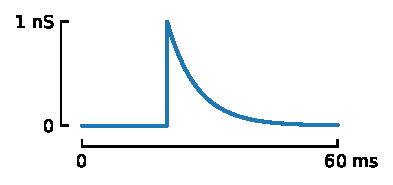
\includegraphics{g1.pdf}
    \captionof{figure}{Example synaptic conductance trace $g_1(t)$, with a single incoming spike at $t = 20$ ms.}
    \label{fig:g1}
}
\marginpar{
    \vspace*{3em}
    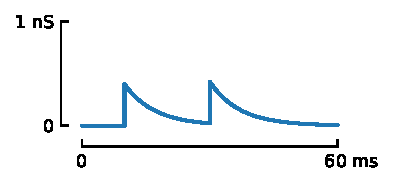
\includegraphics{g2.pdf}
    \captionof{figure}{Another example trace $g_2(t)$, with spikes at $t = 10$ ms and $30$ ms, and a smaller $Δg$.}
    \label{fig:g2}
}

Note that these are not the so called alpha-synapses. Those are two dimensional and also have an exponential rise, instead of just an exponential decay. (For an infinitely fast rise though, these models are of course the same).
Simulating a full alpha synapse might increase the realism of our voltage traces, for a small simulation cost. We did not try this however. Foremost because alpha synapses fit to real data often have very fast rise times that are almost indistinguishable from instantaneous jumps.

For efficiency, we give all our excitatory synapses the same reversal potential, $E_\exc$. Idem for the inhibitory synapses, with $E_\inh$. This allows us to factor the synaptic current sum (\cref{eq:I_syn}) as follows:
\begin{equation}
    I_\syn = (V - E_\exc) \sum_{\exc\ i} g_i \  + \  (V - E_\inh) \sum_{\inh\ i} g_i
    \label{eq:I_syn_factor}
\end{equation}

The sums of conductance signals $g_i(t)$ can also be simplified. Say that the values of $g_i$ at $t = 0$ are $G_i$. The solution to \cref{eq:g_i} (at least in the time until a new presynaptic spike arrives) is then
\begin{equation}
    g_i(t) = G_i\ e^{-t/\tau}
\end{equation}

With this, and when all synapses have the same time constant $\tau$, the two sums in \cref{eq:I_syn_factor} can be factored as follows:\footnotemark
\footnotetext{
    This is only valid in the time before any new spikes arrive.
    To see that the 'summability' still holds after a new spike arrives, the above reasoning can be repeated, but simply with different values for the $G_i$ (all decayed by an amount $e^{-t_\text{spike}/\tau}$, and one increased by a bump $Δg_i$), and then redefining $t_\text{spike}$ to be $t = 0$.
}
\begin{equation}
    \sum_i g_i(t) = \sum_i \left( G_i\ e^{-t/\tau} \right)
                            = \left( \sum_i G_i  \right) e^{-t/\tau}
\end{equation}
This means that we need to only keep track of two conductance signals: $g_\exc$ and $g_\inh$, each the sum of all excitatory or all inhibitory synaptic conductances.

\marginpar{
    \vspace*{2em}
    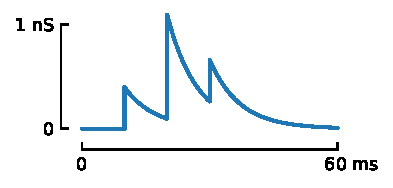
\includegraphics{g3.pdf}
    \captionof{figure}{A third synaptic conductance trace $g_3(t)$, with three input spikes at the same times and strengths as in \cref{fig:g1,fig:g2}. This signal is simulated independently, but turns out to be equal to the sum of the two others: $g_3(t) ≡ g_1(t) + g_2(t)$.}
}

Our synaptic current sum then becomes simply:
\begin{equation}
    I_\syn = (V - E_\exc)\ g_\exc \  + \  (V - E_\inh)\ g_\inh,
\end{equation}
and we only need to simulate two differential equations, instead of one for every synapse:
\begin{align*}
    \d{g_\exc} &= -g_\exc / \tau \\
    \d{g_\inh} &= -g_\inh / \tau,
\end{align*}
where on arrival of a spike at synapse $i$ either $g_\exc$ or $g_\inh$ is instantaneously increased by a value $Δg_i$, depending on whether that synapse is excitatory or inhibitory.


\section{Input spikes}

In our simplest experimental setup, we simulate just one AdEx neuron.
Its input is provided by an array of $N$ Poisson neurons, i.e. they each generate spike trains according to a Poisson process. We call this the `N-to-1' setup.

The inter-event intervals of a Poisson process follow an exponential distribution.
We use that fact to generate spike trains: we draw samples from $\mathrm{Exp}(\lambda)$ (with $\lambda$ the desired firing rate), and cumulatively sum up these intervals  to obtain spike times. This is done until we have reached the desired input train duration.


\section{Voltage imaging}

The signals detected by a light microscope in a voltage imaging setup are not the same as the real membrane voltage signals of which they are a reflection.

We model this lossy transformation by simply adding Gaussian noise to our simulated membrane voltage. As in the voltage imaging literature, we quantify the amount of this  noise by a `spike-SNR' measure (spike signal-to-noise ratio). This is defined as the height of an average spike relative to the standard deviation of the noise.

A more realistic model of the voltage-imaging transformation would also incorporate the exponential decay over time of the SNR, and the short-term 'smearing in time' of voltage indicators. The latter could be done by passing the voltage signal through a linear filter with some non-instantaneous impulse response.
